\section{26th February 2023: Seven Trumpets}
\subsection*{Text: Revelation 8:1-9:21, 11:14-19}
  \begin{quote}
    [1] When the Lamb opened the seventh seal, there was silence in heaven for about half an hour. [2] Then I saw the seven angels who stand before God, and seven trumpets were given to them. [3] And another angel came and stood at the altar with a golden censer, and he was given much incense to offer with the prayers of all the saints on the golden altar before the throne, [4] and the smoke of the incense, with the prayers of the saints, rose before God from the hand of the angel. [5] Then the angel took the censer and filled it with fire from the altar and threw it on the earth, and there were peals of thunder, rumblings, flashes of lightning, and an earthquake.

    [6] Now the seven angels who had the seven trumpets prepared to blow them.

    [7] The first angel blew his trumpet, and there followed hail and fire, mixed with blood, and these were thrown upon the earth. And a third of the earth was burned up, and a third of the trees were burned up, and all green grass was burned up.

    [8] The second angel blew his trumpet, and something like a great mountain, burning with fire, was thrown into the sea, and a third of the sea became blood. [9] A third of the living creatures in the sea died, and a third of the ships were destroyed.

    [10] The third angel blew his trumpet, and a great star fell from heaven, blazing like a torch, and it fell on a third of the rivers and on the springs of water. [11] The name of the star is Wormwood. A third of the waters became wormwood, and many people died from the water, because it had been made bitter.

    [12] The fourth angel blew his trumpet, and a third of the sun was struck, and a third of the moon, and a third of the stars, so that a third of their light might be darkened, and a third of the day might be kept from shining, and likewise a third of the night.

    [13] Then I looked, and I heard an eagle crying with a loud voice as it flew directly overhead, “Woe, woe, woe to those who dwell on the earth, at the blasts of the other trumpets that the three angels are about to blow!”

    [1] And the fifth angel blew his trumpet, and I saw a star fallen from heaven to earth, and he was given the key to the shaft of the bottomless pit. [2] He opened the shaft of the bottomless pit, and from the shaft rose smoke like the smoke of a great furnace, and the sun and the air were darkened with the smoke from the shaft. [3] Then from the smoke came locusts on the earth, and they were given power like the power of scorpions of the earth. [4] They were told not to harm the grass of the earth or any green plant or any tree, but only those people who do not have the seal of God on their foreheads. [5] They were allowed to torment them for five months, but not to kill them, and their torment was like the torment of a scorpion when it stings someone. [6] And in those days people will seek death and will not find it. They will long to die, but death will flee from them.

    [7] In appearance the locusts were like horses prepared for battle: on their heads were what looked like crowns of gold; their faces were like human faces, [8] their hair like women’s hair, and their teeth like lions’ teeth; [9] they had breastplates like breastplates of iron, and the noise of their wings was like the noise of many chariots with horses rushing into battle. [10] They have tails and stings like scorpions, and their power to hurt people for five months is in their tails. [11] They have as king over them the angel of the bottomless pit. His name in Hebrew is Abaddon, and in Greek he is called Apollyon.

    [12] The first woe has passed; behold, two woes are still to come.

    [13] Then the sixth angel blew his trumpet, and I heard a voice from the four horns of the golden altar before God, [14] saying to the sixth angel who had the trumpet, “Release the four angels who are bound at the great river Euphrates.” [15] So the four angels, who had been prepared for the hour, the day, the month, and the year, were released to kill a third of mankind. [16] The number of mounted troops was twice ten thousand times ten thousand; I heard their number. [17] And this is how I saw the horses in my vision and those who rode them: they wore breastplates the color of fire and of sapphire and of sulfur, and the heads of the horses were like lions’ heads, and fire and smoke and sulfur came out of their mouths. [18] By these three plagues a third of mankind was killed, by the fire and smoke and sulfur coming out of their mouths. [19] For the power of the horses is in their mouths and in their tails, for their tails are like serpents with heads, and by means of them they wound.

    [20] The rest of mankind, who were not killed by these plagues, did not repent of the works of their hands nor give up worshiping demons and idols of gold and silver and bronze and stone and wood, which cannot see or hear or walk, [21] nor did they repent of their murders or their sorceries or their sexual immorality or their thefts.

    [14] The second woe has passed; behold, the third woe is soon to come.

    [15] Then the seventh angel blew his trumpet, and there were loud voices in heaven, saying, “The kingdom of the world has become the kingdom of our Lord and of his Christ, and he shall reign forever and ever.” [16] And the twenty-four elders who sit on their thrones before God fell on their faces and worshiped God, [17] saying,

    “We give thanks to you, Lord God Almighty,
        who is and who was,
    for you have taken your great power
        and begun to reign.
    [18] The nations raged,
        but your wrath came,
        and the time for the dead to be judged,
    and for rewarding your servants, the prophets and saints,
        and those who fear your name,
        both small and great,
    and for destroying the destroyers of the earth.”

    [19] Then God’s temple in heaven was opened, and the ark of his covenant was seen within his temple. There were flashes of lightning, rumblings, peals of thunder, an earthquake, and heavy hail.

  \end{quote}
\subsection*{Notes}
\begin{itemize}
  \item{What are the relationships between the seals, trumpets and bowls?
  Are they describing the same set of judgment in three different ways?  Or
  are they describing different judgments?  For our church, we shall take
  there to be three set of judgments that all end together with the vision
  around the throne.  Like, the seven trumpets are part of the seventh seal,
  and the seven bowls are part of the seventh trumpets.  And thus when the
  bowls end, the trumpets also end and hence the seals also end (see Figure~\ref{fig: r/s between seals, trumpets and bowls}). 
  
  \begin{figure}[H]
    \centering
    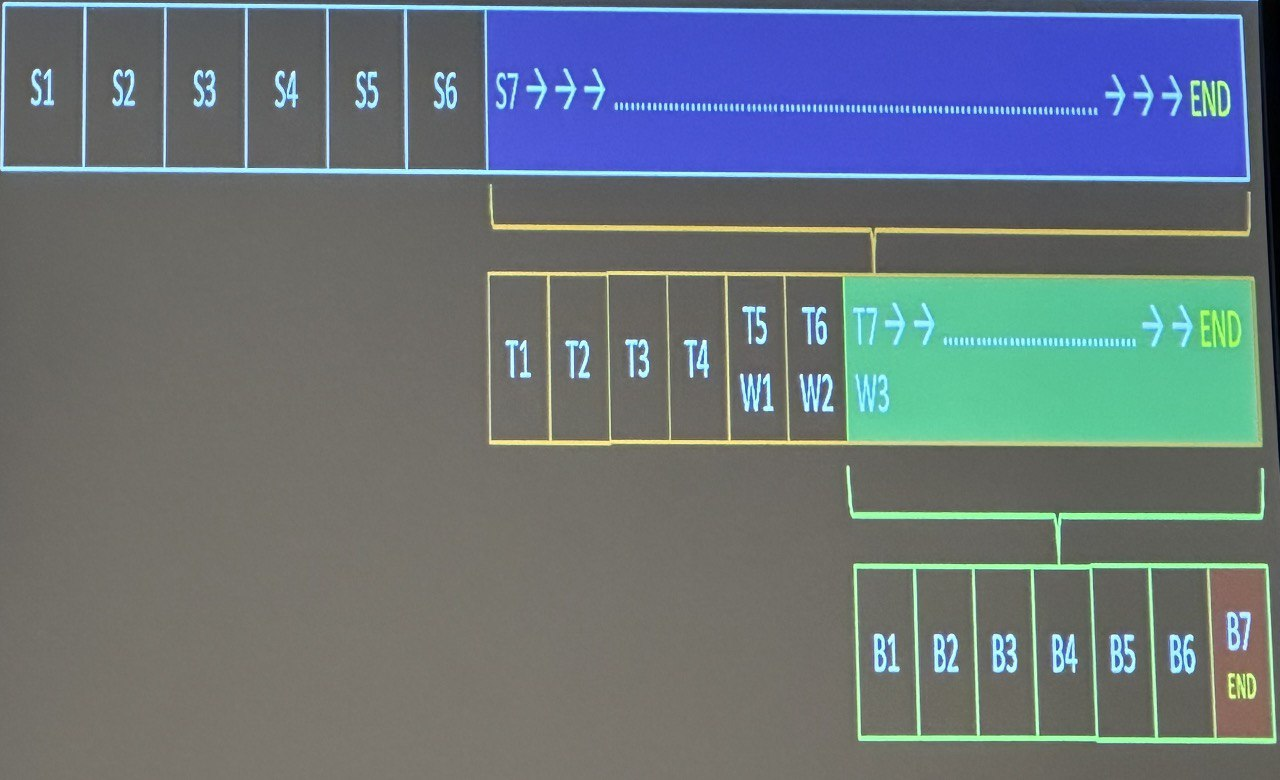
\includegraphics[width=0.6\textwidth, trim={0cm 0cm 0cm 0cm},clip]{Figures/febSermon4Fig1}
    \caption[]{Relationship between the seven seals, seven trumpets and seven bowls.}
    \label{fig: r/s between seals, trumpets and bowls}
  \end{figure}
  
  }

  \item{Trumpets had many uses in the OT.  Trumpets, in Joel 2:1, announces
  the ``day of the Lord''.  Trumpets also in 1 Kings denote the crowning of a
  new king.  Trumpets are also a call to bring together the people (Numbers
  10:2-4), and to warn and to call to war (Numbers 10:9).  Trumpets also were
  used in worship.  So here, the trumpets serve to warn the people of the
  earth that a new king has been crowned, and then judgment (and war) is
  coming.  For the people of the world, it is a call to repent.  And for
  those who have been sealed, it is a call to worship God for His righteous
  judgment.  }
  \item{The water turning into blood is a throwback to the ten plagues during
  the Exodus.  Actually a lot of the trumpets are throwbacks to the ten
  plagues (quite clear in the first four trumpets).  }
  \item{For us, we must remember that our prayers are heard by God, and they
  do rise like incense before God's throne.  Blessed are who seek for God's
  righteousness, for they will be satisfied, as per the Beautitudes.}
  \item{The next three trumpets were described as three woes.  For the fifth
  trumpet, we see that the key to the bottomless pit was given to the star
  fallen from heaven to earth.  If we recall, Jesus has the keys to death and
  the grave.  Hence, we know Jesus is still in control.  Anyway, the locust
  plagues in the first woe is again a throwback to the Exodus.  Also, the
  imagery of locusts come from Joel.  The king of the locusts is called
  ``Abbadon'' or ``Apollyon''.  These locusts, unlike actual locusts, don't
  destroy crops, but they were sent to torment (but not kill) those who
  weren't sealed with the seal of God (c.f Revelation 7).  For the sixth
  trumpet, we have death.  This again is a throwback to the ten plagues in
  the Exodus event.  }
  \item{Just like how there was an interlude after the sixth seal and before
  the seventh seal, there is also an interlude after the sixth trumpet and
  before the seventh trumpet. The interlude here is in chapter 10 and in the first half of chapter 11.}
  \item{Now, the scary thing is that after the sixth trumpet, even while God
  is judging, the unsealed people still alive still don't repent.  They are
  still committing their evil deeds.  For us today, how should we respond to
  these six trumpets?  As Hebrews says, ``How shall we escape if we neglect
  so great a salvation''?  We must keep watch of our soul and make sure that
  no root of bitterness springs up like Esau, so that on the day of the Lord,
  we may be found to be sealed.  }
  \item{After the seventh trumpet was blown, we have a proclamation of
  victory and worship in heaven.  Here, we see the ark of the covenant, which
  is a reminder of God's presence with His people.  Hence, we can be assured
  that if we are on Jesus' side, we don't need to be afraid of all of these
  judgments.  And then we also see lightings, rumblings, peals of thunder,
  earthquake and heavy hail, which are related to the prayers of the saints.}
  \item{In conclusion, today's sermon had three points:
  \begin{enumerate}
    \item{\textbf{A}ngels and trumpets}
    \item{\textbf{E}ffects of judgment}
    \item{\textbf{D}eclaration of victory}
  \end{enumerate}
  Just like an AED, if our hearts are dead today, hopefully today's message of judgment will wake us up and cause us to repent, lest we be found among the unsealed people on the day of judgment.}
\end{itemize}